\section{Performance test}
This section contains the results from the performance test done by the subjects. First of the results from the regressor trained only with EMG data are presented, and afterwards compared to the regressor trained with inclusion of IMU data. The bar chart in \ref{fig:GotItTime} shows the performance scores of all limb positions for both features.

\begin{figure}[H]
	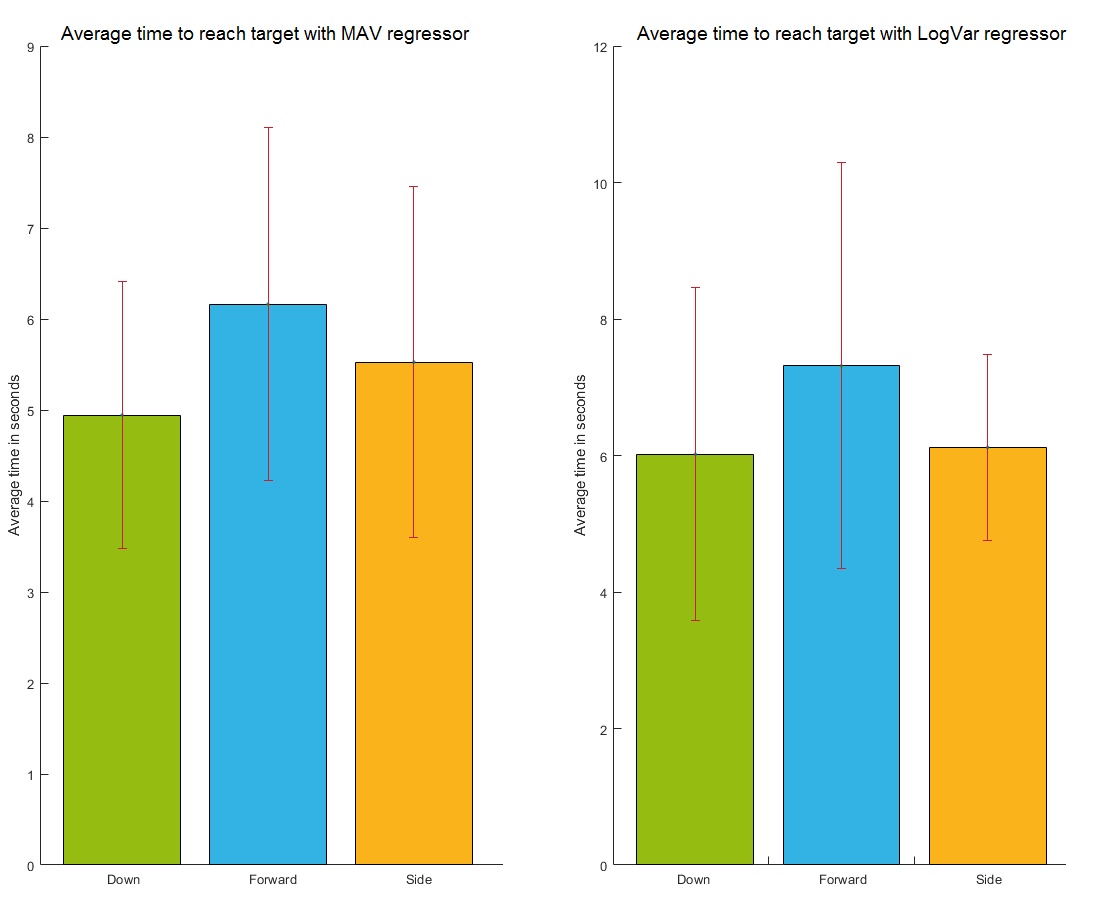
\includegraphics[width=0.7\textwidth]{figures/results/GotItTime}  %<--but is not needed.
	\caption{Calculated performance scores of the regressors. The bar chart illustrates the mean score across all subjects across limb positions, and the error bar illustrates the standard deviation}
	\label{fig:GotItTime}  %<--give the figure a label, so you can reference!
\end{figure}

	\begin{center}
		\begin{tabular}{l l l}
			\toprule
			\textbf{Limb position and feature} & \textbf{Performance score} & \textbf{Standard deviation}\\
			\midrule
			Down, MAV & 5.34 & $\pm 1.57$ \\
			Forward, MAV & 8.18 & $\pm 4.71$ \\
			Side, MAV & 6.05 & $\pm 2.05$ \\
			Down, LogVar & 6.54 & $\pm 2.53$ \\
			Forward, LogVar & 7.91 & $\pm 3.46$ \\
			Side, LogVar & 6.93 & $\pm 2.30$ \\
			\bottomrule
		\end{tabular}
		\captionof{table}{Performance scores across limb for MAV and LogVar regressors.}
	\end{center}
	
	\begin{center}
		\begin{tabular}{l l}
			\toprule
			\textbf{Feature} & \textbf{P-Value}\\
			\midrule
			MAV & 0.03 \\
			LogVar & 0.46 \\
			\bottomrule
		\end{tabular}
		\captionof{table}{P-Values for comparison of the performance score across limb positions with MAV and LogVar.}
	\end{center}

A one-sample Kolmogorov-Smirnov test was done on the scores from the MAV and LogVar respectively and showed no normality in both performance score sets (p < 0.001, p < 0.001). A Friedman's test was therefore applied for statistical analysis. The performance scores between the three limb positions prove not to be significantly different (p = 0.46), when applying the LogVar trained regressors in the online test. For the MAV trained regressors the performance score between all limb positions can be proven significantly different (p = 0.03). 

\begin{figure}[H]
	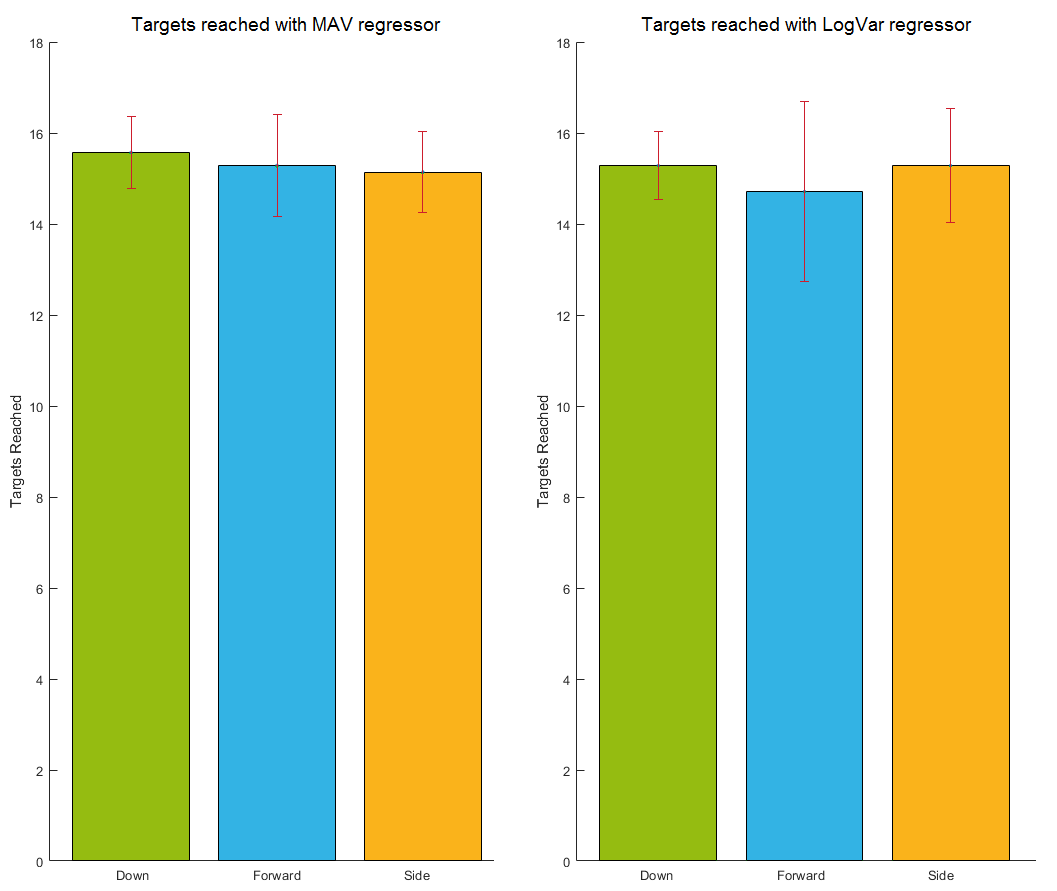
\includegraphics[width=0.7\textwidth]{figures/results/TargetsReached}  %<--but is not needed.
	\caption{The bar chart illustrates the amount of targets reached for the respective limb positions for both features.}
	\label{fig:TargetsReached}  %<--give the figure a label, so you can reference!
\end{figure}

	\begin{center}
		\begin{tabular}{l l l}
			\toprule
			\textbf{Limb position and feature} & \textbf{Overall TR} & \textbf{Standard deviation}\\
			\midrule
			Down, MAV & 15.56 & $\pm 0.73$ \\
			Forward, MAV & 15.11 & $\pm 1.05$ \\
			Side, MAV & 15.22 & $\pm 0.83$ \\
			Down, LogVar & 15.44 & $\pm 0.73$ \\
			Forward, LogVar & 15 & $\pm 1.80$ \\
			Side, LogVar & 15.33 & $\pm 1.12$ \\
			\bottomrule
		\end{tabular}
		\captionof{table}{Targets reached (TR) in the target reaching test with the MAV and LogVar regressors.}
	\end{center}

	\begin{center}
		\begin{tabular}{l l}
			\toprule
			\textbf{Feature} & \textbf{P-Value}\\
			\midrule
			MAV & 0.23 \\
			LogVar & 0.78 \\
			\bottomrule
		\end{tabular}
		\captionof{table}{P-Values for comparison of the number of reached targets across limb positions with MAV and LogVar.}
	\end{center}
	
The Friedman's statistical test shows no significant difference (p = 0.23) between the number of targets reached across limb positions for the MAV regressor. There was no significant difference (p = 0.78) between the limb positions for the LogVar regressor either.

%A qualitative examination of the box plot in \ref{fig:TargetsReached} shows no significant difference in targets reached between limb positions and between all limb positions for the two features, which is similar to the Friedman's test results for the time per reached target.

\begin{figure}[H]
	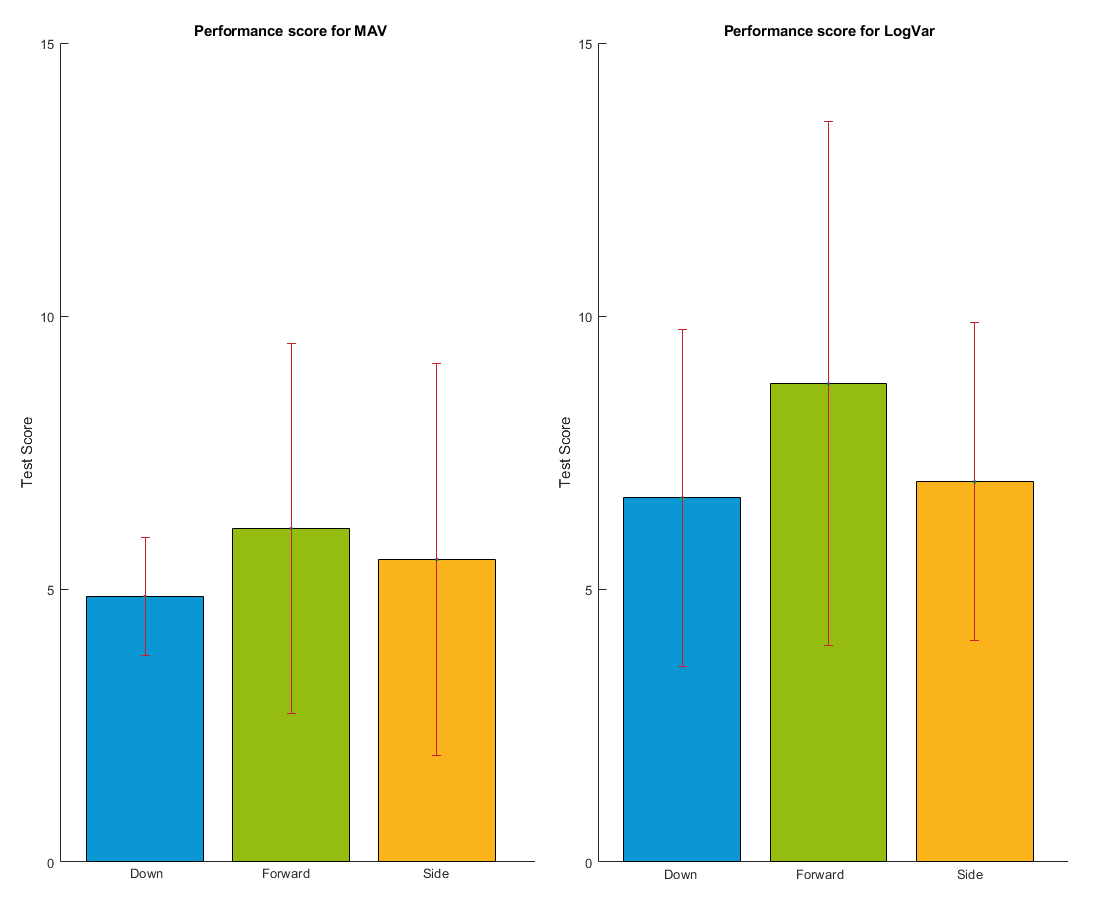
\includegraphics[width=0.7\textwidth]{figures/results/GotItTimeIMU}  %<--but is not needed.
	\caption{Calculated performance scores of the regressors with IMU data included. The bar chart illustrates the mean score across all subjects in the limb positions, and the error bar illustrates the standard deviation.}
	\label{fig:gotItTimeIMU}  %<--give the figure a label, so you can reference!
\end{figure}

	\begin{center}
		\begin{tabular}{l l l}
			\toprule
			\textbf{Limb position and feature} & \textbf{Performance score} & \textbf{Standard deviation}\\
			\midrule
			Down, MAV & 4.87 & $\pm 1.08$ \\
			Forward, MAV & 6.11 & $\pm 3.39$ \\
			Side, MAV & 5.54 & $\pm 3.58$ \\
			Down, LogVar & 6.67 & $\pm 3.08$ \\
			Forward, LogVar & 8.76 & $\pm 4.80$ \\
			Side, LogVar & 6.97 & $\pm 2.91$ \\
			\bottomrule
		\end{tabular}
		\captionof{table}{Performance scores across limb positions for MAV and LogVar regressors with IMU included.}
	\end{center}
	
		\begin{center}
			\begin{tabular}{l l}
				\toprule
				\textbf{Feature} & \textbf{P-Value}\\
				\midrule
				MAV & 0.90 \\
				LogVar & 0.24 \\
				\bottomrule
			\end{tabular}
			\captionof{table}{P-Values for comparison of the performance score across limb positions with MAV and LogVar with IMU data included.}
		\end{center}

The test with IMU data included shows no significant difference (p = 0.90) between the performance score across limb positions for the MAV regressor. No difference was proven in the LogVar test (p = 0.24) either.

\begin{figure}[H]
	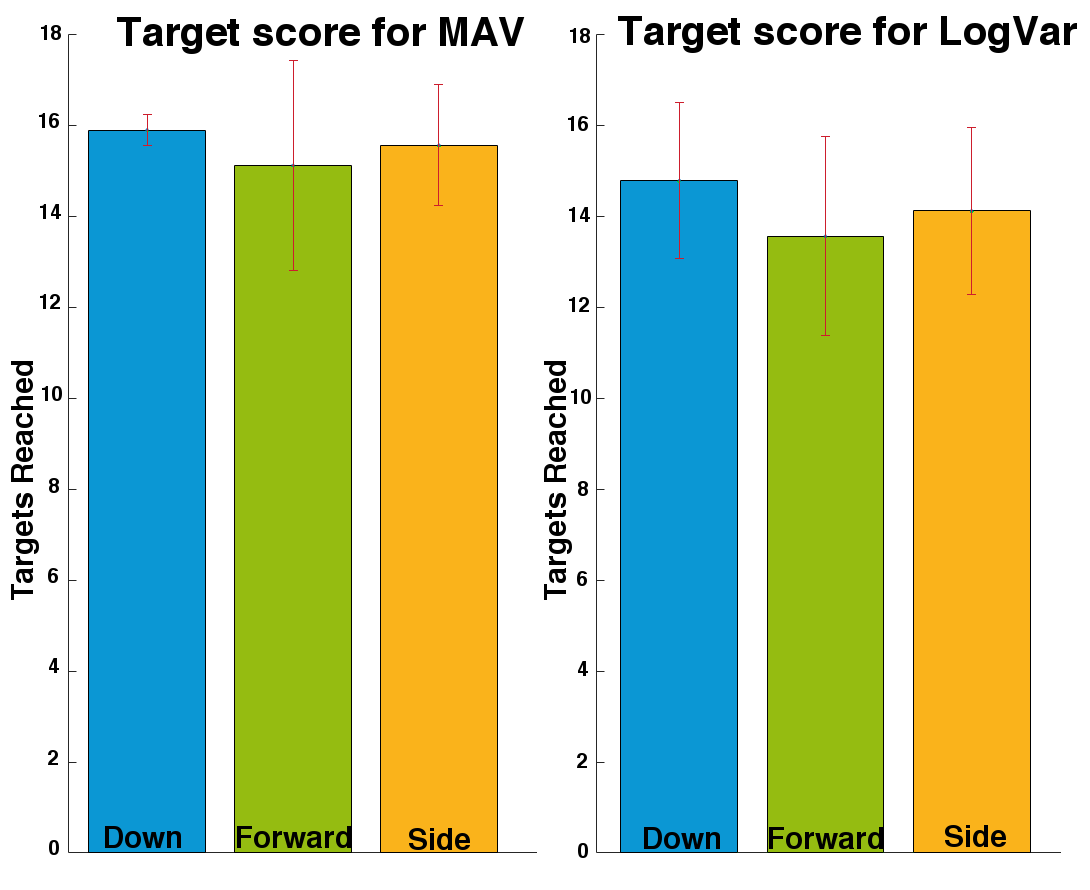
\includegraphics[width=0.7\textwidth]{figures/results/TargetsReachedIMU}  %<--but is not needed.
	\caption{The bar chart illustrates the amount of targets reached for the respective limb positions for both features with IMU data included.}
	\label{fig:TargetsReachedIMU}  %<--give the figure a label, so you can reference!
\end{figure}

	\begin{center}
		\begin{tabular}{l l l}
			\toprule
			\textbf{Limb position and feature} & \textbf{Overall TR} & \textbf{Standard deviation}\\
			\midrule
			Down, MAV & 15.89 & $\pm 0.33$ \\
			Forward, MAV & 15.11 & $\pm 2.32$ \\
			Side, MAV & 15.56 & $\pm 1.33$ \\
			Down, LogVar & 14.78 & $\pm 1.72$ \\
			Forward, LogVar & 13.56 & $\pm 2.19$ \\
			Side, LogVar & 14.11 & $\pm 1.83$ \\
			\bottomrule
		\end{tabular}
		\captionof{table}{Targets reached (TR) in the target reaching test with the MAV and LogVar regressors with IMU data included.}
	\end{center}
	
	\begin{center}
		\begin{tabular}{l l}
			\toprule
			\textbf{Compared Features} & \textbf{P-Value}\\
			\midrule
			MAV & 0.50 \\
			LogVar & 0.10 \\
			\bottomrule
		\end{tabular}
		\captionof{table}{P-Values for comparison of the number of targets reached across limb positions with MAV and LogVar with IMU data included.}
	\end{center}
	
The number of targets reached across limb positions can be proven to be significantly different (p = 0.10) for the LogVar feature with IMU data included, where the lowest number of targets reached (mean = 13.56) was found when the subjects pointed their arm forward. There was no significant difference found for the MAV regressor with IMU data included (p = 0.50).
	
\subsection{Comparison of regressors with and without IMU data}

\begin{figure}[H]
	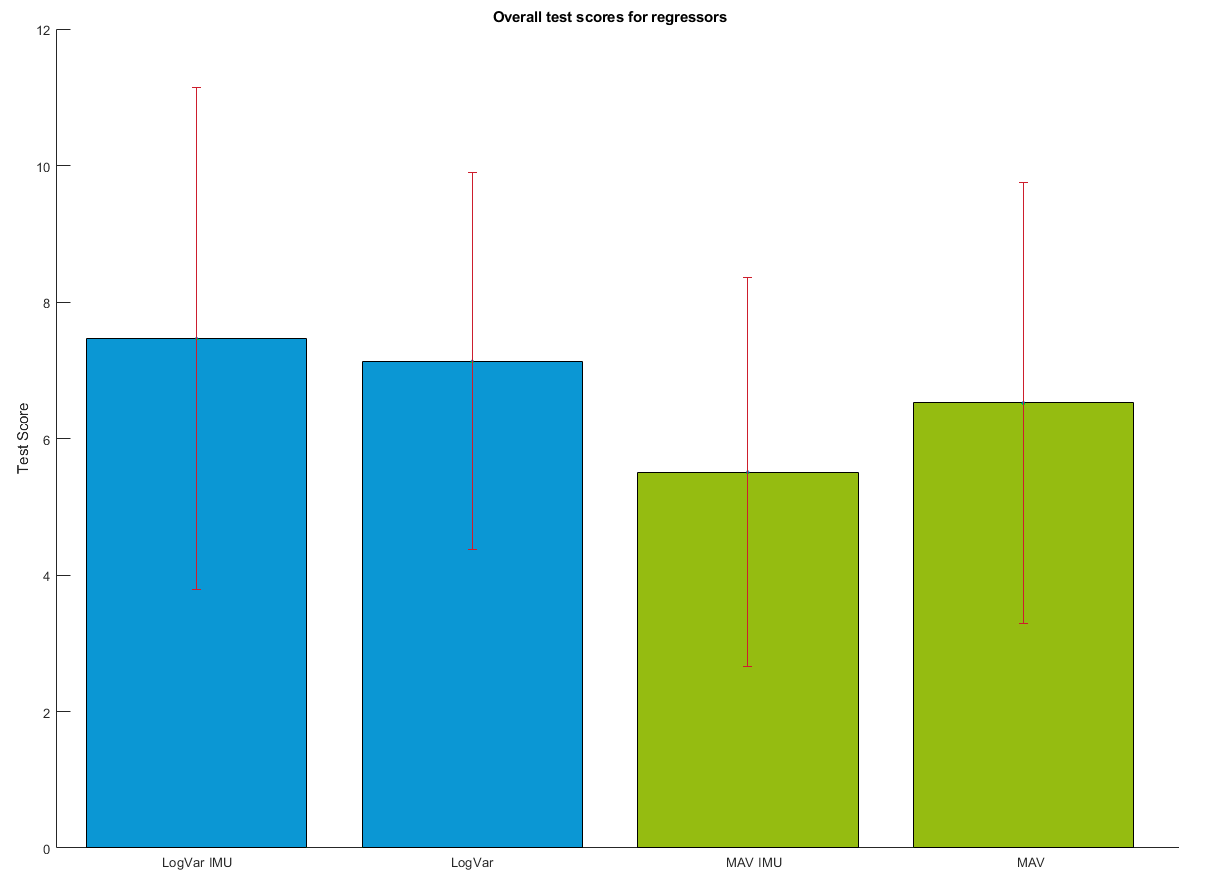
\includegraphics[width=0.7\textwidth]{figures/results/allRegressorBarzTimeScoreForTargetTest}  %<--but is not needed.
	\caption{Calculated overall performance scores of the regressors with and without IMU data included. The bar chart illustrates the mean score across all subjects, and the error bar illustrates the standard deviation}
	\label{fig:gotItTimeOverall}  %<--give the figure a label, so you can reference!
\end{figure}

\begin{center}
	\begin{tabular}{l l l}
		\toprule
		\textbf{Feature} & \textbf{Mean score} & \textbf{Standard deviation}\\
		\midrule
		MAV & 6.52 & $\pm 3.23$ \\
		MAV w. IMU & 5.51 & $\pm 2.85$ \\
		LogVar & 7.13 & $\pm 2.76$ \\
		LogVar w. IMU & 7.46 & $\pm 3.67$ \\
		\bottomrule
	\end{tabular}
	\captionof{table}{Average performance score of the target reaching test for the four regressor designs.}
\end{center}

\begin{center}
	\begin{tabular}{l l}
		\toprule
		\textbf{Compared features} & \textbf{P-Value}\\
		\midrule
		LogVar, MAV & 0.08 \\
		LogVar w. IMU, MAV w. IMU & 0.56 \\
		MAV w. IMU, MAV & 0.18 \\
		LogVar w. IMU, LogVar & 0.56 \\
		\bottomrule
	\end{tabular}
	\captionof{table}{P-Values for comparison of the overall performance scores of the target reaching tests.}
\end{center}

When comparing all performance scores from the two feature trained regression control schemes without IMU, the Friedman's test proves no significant difference (LogVar: 7.13 s, MAV: 6.52 s; p = 0.08). There is no significant difference to be found between LogVar and MAV with IMU data included (LogVar w. IMU: 7.46, MAV w. IMU: 5.51, p = 0.56), and no difference was found between features with and without IMU for either MAV (wo. IMU: 6.5219, w. IMU: 5.5066, p = 0.1779) or LogVar (wo. IMU: 7.1284, w. IMU: 7.4646, p = 0.5637).


\begin{figure}[H]
	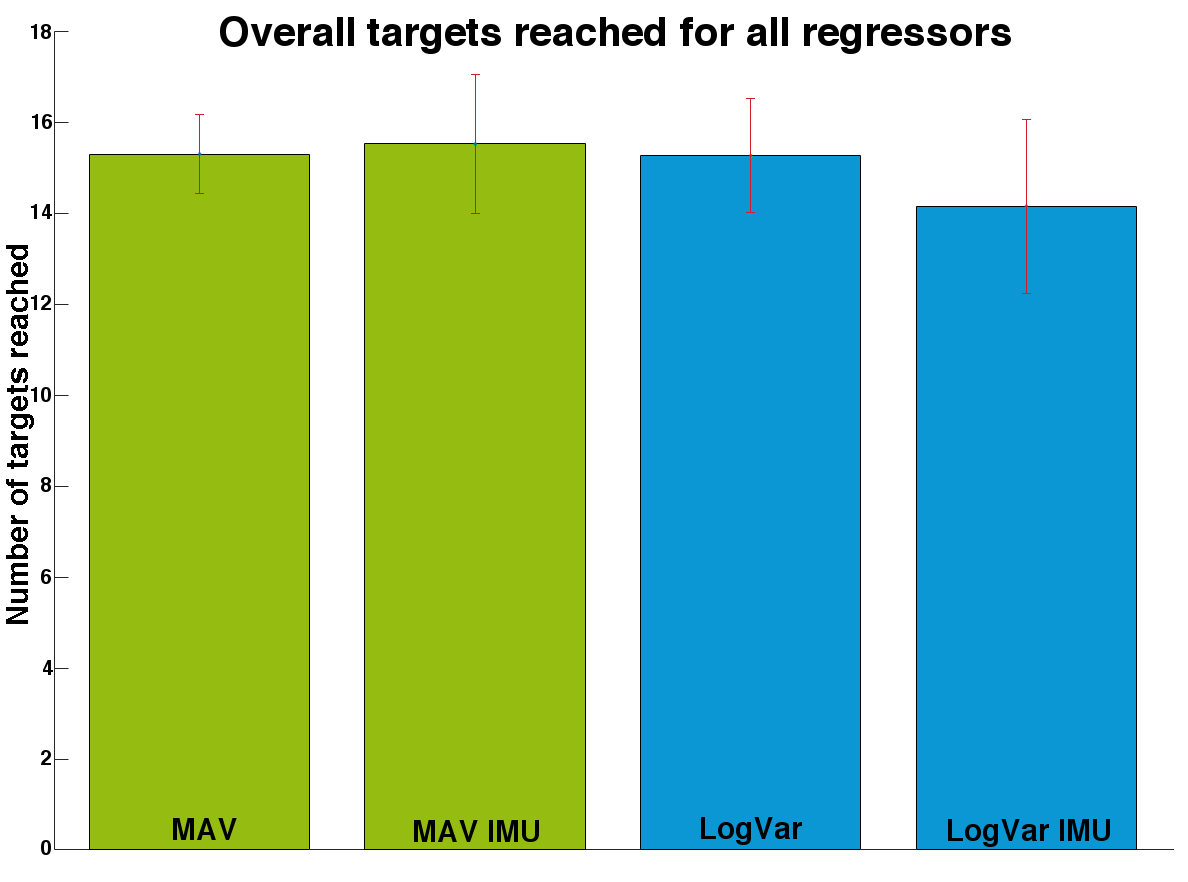
\includegraphics[width=0.7\textwidth]{figures/results/sumMoreBarsWithTargetsReachedForAllRegressors}  %<--but is not needed.
	\caption{The bar chart illustrates the amount of targets reached for all limb positions for the two features with and without IMU data included.}
	\label{fig:TargetsReachedOverall}  %<--give the figure a label, so you can reference!
\end{figure}

\begin{center}
	\begin{tabular}{l l l}
		\toprule
		\textbf{Feature} & \textbf{Overall mean error} & \textbf{Standard deviation}\\
		\midrule
		MAV & 15.2963 & $\pm 0.8689$ \\
		MAV w. IMU & 15.5185 & $\pm 1.5285$ \\
		LogVar & 15.2593 & $\pm 1.2586$ \\
		LogVar w. IMU & 14.1481 & $\pm 1.9156$ \\
		\bottomrule
	\end{tabular}
	\captionof{table}{Average number of targets reached in the target reaching test for the four regressor designs.}
\end{center}

		
\begin{center}
	\begin{tabular}{l l}
		\toprule
			\textbf{Compared Features} & \textbf{P-Value}\\
			\midrule
			LogVar, MAV & 1 \\
			LogVar w/ IMU, MAV w/ IMU & 0.0017 \\
			MAV, MAV w/ IMU & 0.0124 \\
			LogVar, LogVar w/ IMU & 0.0016 \\
			\bottomrule
	\end{tabular}
	\captionof{table}{P-Values for comparison targets reached in the target reaching tests.}
\end{center}

A significant difference was found between LogVar and MAV when IMU was included (LogVar w. IMU: 14.1481, MAV w. IMU: 15.5185, p = 0.0017), and the same was found when including IMU data for both MAV (wo. IMU: 15.2963, w. IMU: 15.5185, p = 0.0124) and LogVar (wo. IMU: 15.2593, w. IMU: 14.1481, p = 0.0016). The performance was similar when comparing the overall number of targets reached for LogVar and MAV (p = 1).